% Options for packages loaded elsewhere
\PassOptionsToPackage{unicode}{hyperref}
\PassOptionsToPackage{hyphens}{url}
%
\documentclass[
]{article}
\usepackage{amsmath,amssymb}
\usepackage{iftex}
\ifPDFTeX
  \usepackage[T1]{fontenc}
  \usepackage[utf8]{inputenc}
  \usepackage{textcomp} % provide euro and other symbols
\else % if luatex or xetex
  \usepackage{unicode-math} % this also loads fontspec
  \defaultfontfeatures{Scale=MatchLowercase}
  \defaultfontfeatures[\rmfamily]{Ligatures=TeX,Scale=1}
\fi
\usepackage{lmodern}
\ifPDFTeX\else
  % xetex/luatex font selection
\fi
% Use upquote if available, for straight quotes in verbatim environments
\IfFileExists{upquote.sty}{\usepackage{upquote}}{}
\IfFileExists{microtype.sty}{% use microtype if available
  \usepackage[]{microtype}
  \UseMicrotypeSet[protrusion]{basicmath} % disable protrusion for tt fonts
}{}
\makeatletter
\@ifundefined{KOMAClassName}{% if non-KOMA class
  \IfFileExists{parskip.sty}{%
    \usepackage{parskip}
  }{% else
    \setlength{\parindent}{0pt}
    \setlength{\parskip}{6pt plus 2pt minus 1pt}}
}{% if KOMA class
  \KOMAoptions{parskip=half}}
\makeatother
\usepackage{xcolor}
\usepackage[margin=1in]{geometry}
\usepackage{color}
\usepackage{fancyvrb}
\newcommand{\VerbBar}{|}
\newcommand{\VERB}{\Verb[commandchars=\\\{\}]}
\DefineVerbatimEnvironment{Highlighting}{Verbatim}{commandchars=\\\{\}}
% Add ',fontsize=\small' for more characters per line
\usepackage{framed}
\definecolor{shadecolor}{RGB}{248,248,248}
\newenvironment{Shaded}{\begin{snugshade}}{\end{snugshade}}
\newcommand{\AlertTok}[1]{\textcolor[rgb]{0.94,0.16,0.16}{#1}}
\newcommand{\AnnotationTok}[1]{\textcolor[rgb]{0.56,0.35,0.01}{\textbf{\textit{#1}}}}
\newcommand{\AttributeTok}[1]{\textcolor[rgb]{0.13,0.29,0.53}{#1}}
\newcommand{\BaseNTok}[1]{\textcolor[rgb]{0.00,0.00,0.81}{#1}}
\newcommand{\BuiltInTok}[1]{#1}
\newcommand{\CharTok}[1]{\textcolor[rgb]{0.31,0.60,0.02}{#1}}
\newcommand{\CommentTok}[1]{\textcolor[rgb]{0.56,0.35,0.01}{\textit{#1}}}
\newcommand{\CommentVarTok}[1]{\textcolor[rgb]{0.56,0.35,0.01}{\textbf{\textit{#1}}}}
\newcommand{\ConstantTok}[1]{\textcolor[rgb]{0.56,0.35,0.01}{#1}}
\newcommand{\ControlFlowTok}[1]{\textcolor[rgb]{0.13,0.29,0.53}{\textbf{#1}}}
\newcommand{\DataTypeTok}[1]{\textcolor[rgb]{0.13,0.29,0.53}{#1}}
\newcommand{\DecValTok}[1]{\textcolor[rgb]{0.00,0.00,0.81}{#1}}
\newcommand{\DocumentationTok}[1]{\textcolor[rgb]{0.56,0.35,0.01}{\textbf{\textit{#1}}}}
\newcommand{\ErrorTok}[1]{\textcolor[rgb]{0.64,0.00,0.00}{\textbf{#1}}}
\newcommand{\ExtensionTok}[1]{#1}
\newcommand{\FloatTok}[1]{\textcolor[rgb]{0.00,0.00,0.81}{#1}}
\newcommand{\FunctionTok}[1]{\textcolor[rgb]{0.13,0.29,0.53}{\textbf{#1}}}
\newcommand{\ImportTok}[1]{#1}
\newcommand{\InformationTok}[1]{\textcolor[rgb]{0.56,0.35,0.01}{\textbf{\textit{#1}}}}
\newcommand{\KeywordTok}[1]{\textcolor[rgb]{0.13,0.29,0.53}{\textbf{#1}}}
\newcommand{\NormalTok}[1]{#1}
\newcommand{\OperatorTok}[1]{\textcolor[rgb]{0.81,0.36,0.00}{\textbf{#1}}}
\newcommand{\OtherTok}[1]{\textcolor[rgb]{0.56,0.35,0.01}{#1}}
\newcommand{\PreprocessorTok}[1]{\textcolor[rgb]{0.56,0.35,0.01}{\textit{#1}}}
\newcommand{\RegionMarkerTok}[1]{#1}
\newcommand{\SpecialCharTok}[1]{\textcolor[rgb]{0.81,0.36,0.00}{\textbf{#1}}}
\newcommand{\SpecialStringTok}[1]{\textcolor[rgb]{0.31,0.60,0.02}{#1}}
\newcommand{\StringTok}[1]{\textcolor[rgb]{0.31,0.60,0.02}{#1}}
\newcommand{\VariableTok}[1]{\textcolor[rgb]{0.00,0.00,0.00}{#1}}
\newcommand{\VerbatimStringTok}[1]{\textcolor[rgb]{0.31,0.60,0.02}{#1}}
\newcommand{\WarningTok}[1]{\textcolor[rgb]{0.56,0.35,0.01}{\textbf{\textit{#1}}}}
\usepackage{longtable,booktabs,array}
\usepackage{calc} % for calculating minipage widths
% Correct order of tables after \paragraph or \subparagraph
\usepackage{etoolbox}
\makeatletter
\patchcmd\longtable{\par}{\if@noskipsec\mbox{}\fi\par}{}{}
\makeatother
% Allow footnotes in longtable head/foot
\IfFileExists{footnotehyper.sty}{\usepackage{footnotehyper}}{\usepackage{footnote}}
\makesavenoteenv{longtable}
\usepackage{graphicx}
\makeatletter
\def\maxwidth{\ifdim\Gin@nat@width>\linewidth\linewidth\else\Gin@nat@width\fi}
\def\maxheight{\ifdim\Gin@nat@height>\textheight\textheight\else\Gin@nat@height\fi}
\makeatother
% Scale images if necessary, so that they will not overflow the page
% margins by default, and it is still possible to overwrite the defaults
% using explicit options in \includegraphics[width, height, ...]{}
\setkeys{Gin}{width=\maxwidth,height=\maxheight,keepaspectratio}
% Set default figure placement to htbp
\makeatletter
\def\fps@figure{htbp}
\makeatother
\setlength{\emergencystretch}{3em} % prevent overfull lines
\providecommand{\tightlist}{%
  \setlength{\itemsep}{0pt}\setlength{\parskip}{0pt}}
\setcounter{secnumdepth}{-\maxdimen} % remove section numbering
\ifLuaTeX
  \usepackage{selnolig}  % disable illegal ligatures
\fi
\IfFileExists{bookmark.sty}{\usepackage{bookmark}}{\usepackage{hyperref}}
\IfFileExists{xurl.sty}{\usepackage{xurl}}{} % add URL line breaks if available
\urlstyle{same}
\hypersetup{
  hidelinks,
  pdfcreator={LaTeX via pandoc}}

\author{}
\date{\vspace{-2.5em}}

\begin{document}

\begin{Shaded}
\begin{Highlighting}[]
\FunctionTok{library}\NormalTok{(ggplot2) }\CommentTok{\# Sert à importer ggplot2 pour avoir plusieurs plots}
\FunctionTok{library}\NormalTok{(dplyr)}
\end{Highlighting}
\end{Shaded}

\begin{verbatim}
## 
## Attaching package: 'dplyr'
\end{verbatim}

\begin{verbatim}
## The following objects are masked from 'package:stats':
## 
##     filter, lag
\end{verbatim}

\begin{verbatim}
## The following objects are masked from 'package:base':
## 
##     intersect, setdiff, setequal, union
\end{verbatim}

\begin{Shaded}
\begin{Highlighting}[]
\FunctionTok{library}\NormalTok{(coin)}
\end{Highlighting}
\end{Shaded}

\begin{verbatim}
## Loading required package: survival
\end{verbatim}

\begin{Shaded}
\begin{Highlighting}[]
\CommentTok{\#initialisation}
\FunctionTok{source}\NormalTok{(}\StringTok{"charger.R"}\NormalTok{)}
\NormalTok{mondata }\OtherTok{\textless{}{-}} \FunctionTok{charger}\NormalTok{(}\DecValTok{2212435}\NormalTok{)}
\end{Highlighting}
\end{Shaded}

\#\#\#\#Phase 1:

\begin{Shaded}
\begin{Highlighting}[]
\DocumentationTok{\#\#\#\#Partie a)}

\CommentTok{\#Histogramme}
\NormalTok{h }\OtherTok{\textless{}{-}}\FunctionTok{hist}\NormalTok{(mondata}\SpecialCharTok{$}\NormalTok{IR, }\AttributeTok{main =} \FunctionTok{paste}\NormalTok{(}\StringTok{"Histogramme de l\textquotesingle{}indice de rugosité"}\NormalTok{), }\AttributeTok{col =} \StringTok{"lightpink"}\NormalTok{, }\AttributeTok{xlab =} \StringTok{" Indice de rugosité (sans unité)"}\NormalTok{, }\AttributeTok{ylab =} \StringTok{"Fréquence"}\NormalTok{, }\AttributeTok{xlim =} \FunctionTok{c}\NormalTok{(}\DecValTok{0}\NormalTok{,}\DecValTok{30}\NormalTok{), }\AttributeTok{ylim =} \FunctionTok{c}\NormalTok{(}\DecValTok{0}\NormalTok{,}\DecValTok{50}\NormalTok{))}
\FunctionTok{text}\NormalTok{(h}\SpecialCharTok{$}\NormalTok{mids,h}\SpecialCharTok{$}\NormalTok{counts,}\AttributeTok{labels=}\NormalTok{h}\SpecialCharTok{$}\NormalTok{counts, }\AttributeTok{adj=}\FunctionTok{c}\NormalTok{(}\FloatTok{0.5}\NormalTok{, }\SpecialCharTok{{-}}\FloatTok{0.5}\NormalTok{))}
\end{Highlighting}
\end{Shaded}

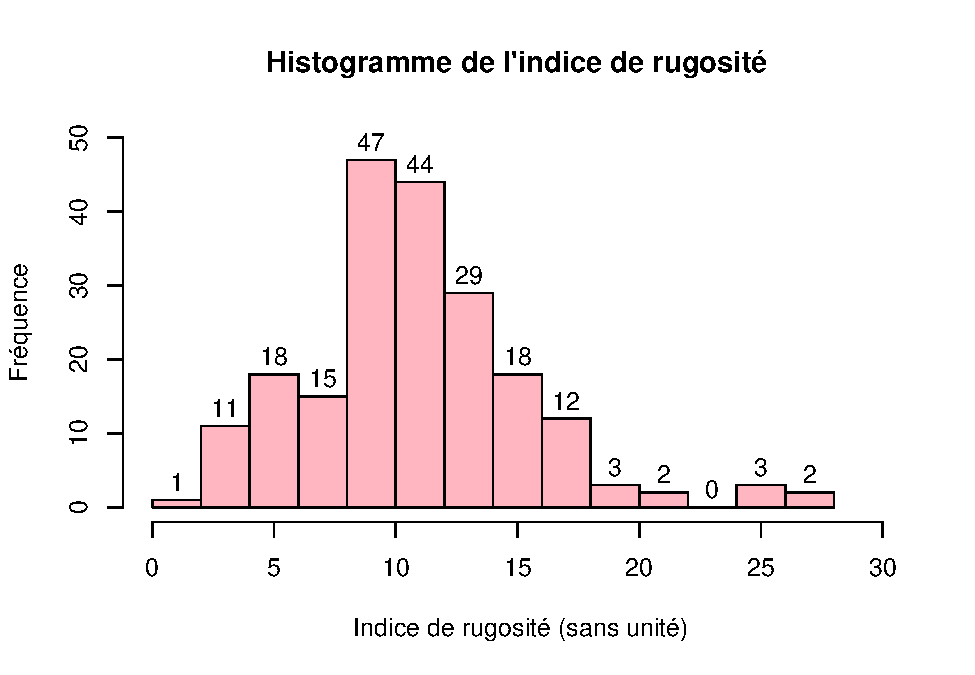
\includegraphics{devoir_files/figure-latex/unnamed-chunk-2-1.pdf}

\begin{Shaded}
\begin{Highlighting}[]
\CommentTok{\#tukey}
\FunctionTok{boxplot}\NormalTok{(mondata}\SpecialCharTok{$}\NormalTok{IR,    }\AttributeTok{main=}\FunctionTok{paste}\NormalTok{(}\StringTok{"Diagramme de tukey de l\textquotesingle{}indice de rugosité"}\NormalTok{),    }\AttributeTok{horizontal=}\NormalTok{T, }\AttributeTok{xlab =} \StringTok{" Indice de rugosité (sans unité)"}\NormalTok{,   }\AttributeTok{col    =}    \StringTok{"lightpink"}\NormalTok{)}
\end{Highlighting}
\end{Shaded}

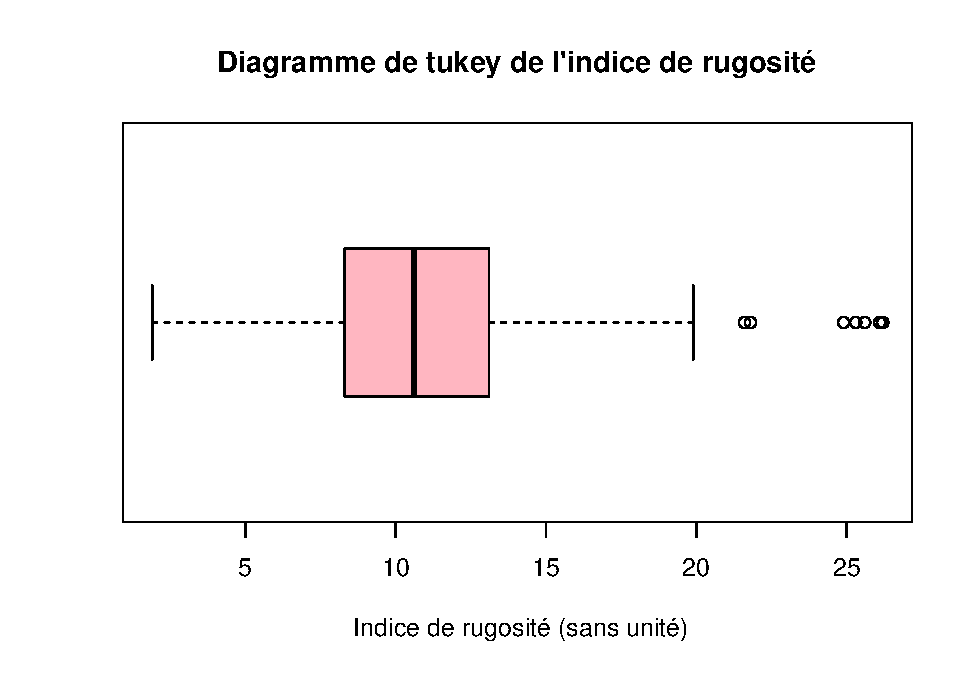
\includegraphics{devoir_files/figure-latex/unnamed-chunk-2-2.pdf}

\begin{Shaded}
\begin{Highlighting}[]
\CommentTok{\#droite de Henry}
\FunctionTok{qqnorm}\NormalTok{(mondata}\SpecialCharTok{$}\NormalTok{IR, }\AttributeTok{col=} \StringTok{"lightpink"}\NormalTok{, }\AttributeTok{main =} \FunctionTok{paste}\NormalTok{(}\StringTok{"Droite de Henry de l\textquotesingle{}indice de rugosité"}\NormalTok{)) }
\FunctionTok{qqline}\NormalTok{(mondata}\SpecialCharTok{$}\NormalTok{IR)}
\end{Highlighting}
\end{Shaded}

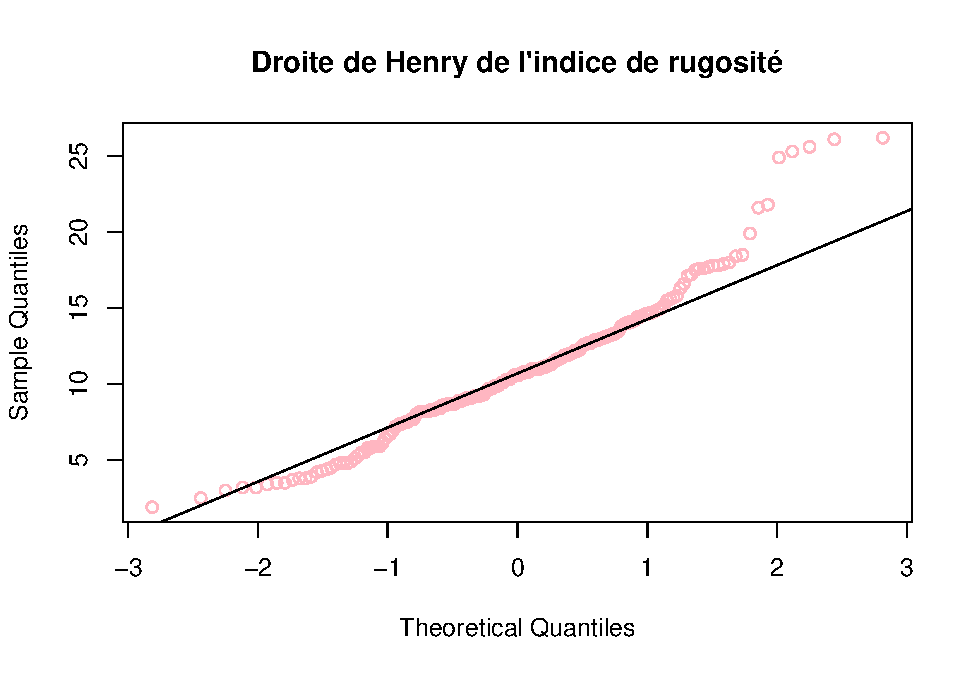
\includegraphics{devoir_files/figure-latex/unnamed-chunk-2-3.pdf}

\begin{Shaded}
\begin{Highlighting}[]
\CommentTok{\#Shapiro}
\FunctionTok{shapiro.test}\NormalTok{(mondata}\SpecialCharTok{$}\NormalTok{IR)}
\end{Highlighting}
\end{Shaded}

\begin{verbatim}
## 
##  Shapiro-Wilk normality test
## 
## data:  mondata$IR
## W = 0.95471, p-value = 4.275e-06
\end{verbatim}

\begin{Shaded}
\begin{Highlighting}[]
\CommentTok{\#tableau statistiques descriptives }
\NormalTok{conf\_int }\OtherTok{\textless{}{-}} \FunctionTok{t.test}\NormalTok{(mondata}\SpecialCharTok{$}\NormalTok{IR)}\SpecialCharTok{$}\NormalTok{conf.int}
\NormalTok{Interval\_Confiance\_Min }\OtherTok{=}\NormalTok{ conf\_int[}\DecValTok{1}\NormalTok{]}
\NormalTok{  Interval\_Confiance\_Max }\OtherTok{=}\NormalTok{ conf\_int[}\DecValTok{2}\NormalTok{]}
\NormalTok{q1 }\OtherTok{\textless{}{-}} \FunctionTok{quantile}\NormalTok{(mondata}\SpecialCharTok{$}\NormalTok{IR, }\FloatTok{0.25}\NormalTok{)}
\NormalTok{q2 }\OtherTok{\textless{}{-}} \FunctionTok{quantile}\NormalTok{(mondata}\SpecialCharTok{$}\NormalTok{IR, }\FloatTok{0.5}\NormalTok{)}
\NormalTok{q3 }\OtherTok{\textless{}{-}} \FunctionTok{quantile}\NormalTok{(mondata}\SpecialCharTok{$}\NormalTok{IR, }\FloatTok{0.75}\NormalTok{)}
\NormalTok{moyenne }\OtherTok{\textless{}{-}} \FunctionTok{mean}\NormalTok{(mondata}\SpecialCharTok{$}\NormalTok{IR)}
\NormalTok{ecart\_type }\OtherTok{\textless{}{-}} \FunctionTok{sd}\NormalTok{(mondata}\SpecialCharTok{$}\NormalTok{IR)}

\NormalTok{dataframe1 }\OtherTok{\textless{}{-}} \FunctionTok{data.frame}\NormalTok{(}
  
\NormalTok{  moyenne,}
\NormalTok{  q1,}
\NormalTok{  q2,}
\NormalTok{  q3,}
\NormalTok{  ecart\_type,}
\NormalTok{  Interval\_Confiance\_Min,}
\NormalTok{  Interval\_Confiance\_Max}

\NormalTok{)}

\NormalTok{knitr}\SpecialCharTok{::}\FunctionTok{kable}\NormalTok{(}\FunctionTok{head}\NormalTok{(dataframe1),}\AttributeTok{caption=}\StringTok{"Tableau des statistiques descriptives sur l\textquotesingle{}indice de rugosité"}\NormalTok{)}
\end{Highlighting}
\end{Shaded}

\begin{longtable}[]{@{}
  >{\raggedright\arraybackslash}p{(\columnwidth - 14\tabcolsep) * \real{0.0476}}
  >{\raggedleft\arraybackslash}p{(\columnwidth - 14\tabcolsep) * \real{0.1071}}
  >{\raggedleft\arraybackslash}p{(\columnwidth - 14\tabcolsep) * \real{0.0476}}
  >{\raggedleft\arraybackslash}p{(\columnwidth - 14\tabcolsep) * \real{0.0595}}
  >{\raggedleft\arraybackslash}p{(\columnwidth - 14\tabcolsep) * \real{0.0595}}
  >{\raggedleft\arraybackslash}p{(\columnwidth - 14\tabcolsep) * \real{0.1310}}
  >{\raggedleft\arraybackslash}p{(\columnwidth - 14\tabcolsep) * \real{0.2738}}
  >{\raggedleft\arraybackslash}p{(\columnwidth - 14\tabcolsep) * \real{0.2738}}@{}}
\caption{Tableau des statistiques descriptives sur l'indice de
rugosité}\tabularnewline
\toprule\noalign{}
\begin{minipage}[b]{\linewidth}\raggedright
\end{minipage} & \begin{minipage}[b]{\linewidth}\raggedleft
moyenne
\end{minipage} & \begin{minipage}[b]{\linewidth}\raggedleft
q1
\end{minipage} & \begin{minipage}[b]{\linewidth}\raggedleft
q2
\end{minipage} & \begin{minipage}[b]{\linewidth}\raggedleft
q3
\end{minipage} & \begin{minipage}[b]{\linewidth}\raggedleft
ecart\_type
\end{minipage} & \begin{minipage}[b]{\linewidth}\raggedleft
Interval\_Confiance\_Min
\end{minipage} & \begin{minipage}[b]{\linewidth}\raggedleft
Interval\_Confiance\_Max
\end{minipage} \\
\midrule\noalign{}
\endfirsthead
\toprule\noalign{}
\begin{minipage}[b]{\linewidth}\raggedright
\end{minipage} & \begin{minipage}[b]{\linewidth}\raggedleft
moyenne
\end{minipage} & \begin{minipage}[b]{\linewidth}\raggedleft
q1
\end{minipage} & \begin{minipage}[b]{\linewidth}\raggedleft
q2
\end{minipage} & \begin{minipage}[b]{\linewidth}\raggedleft
q3
\end{minipage} & \begin{minipage}[b]{\linewidth}\raggedleft
ecart\_type
\end{minipage} & \begin{minipage}[b]{\linewidth}\raggedleft
Interval\_Confiance\_Min
\end{minipage} & \begin{minipage}[b]{\linewidth}\raggedleft
Interval\_Confiance\_Max
\end{minipage} \\
\midrule\noalign{}
\endhead
\bottomrule\noalign{}
\endlastfoot
25\% & 10.85854 & 8.3 & 10.6 & 13.1 & 4.517969 & 10.23638 & 11.48069 \\
\end{longtable}

\#\#\#Explications:

L'histogramme de l'indice de rugosité révèle des caractéristiques
significatives sur la distribution de cette mesure au sein de notre
ensemble de données. Deux classes, 8 \textless{} x \textless{} 10 et 10
\textless{} x \textless{} 12, émergent nettement avec la fréquence la
plus élevée, suggérant que la majorité des observations d'IR se
concentrent dans ces plages.De plus, la dispersion des données n'est pas
uniforme, indiquant des concentrations spécifiques plutôt qu'une
répartition égale. Le centre de la distribution, approximativement à 11,
révèle une tendance centrale significative. Nous pouvons voir avec
l'histogramme et le diagramme de Tukey que la valeur de l'efficacité est
assez bien répartie et que les valeurs sont plus étendues vers la
droite, ce qui explique pourquoi la mediane (q2) est un peu moins élevé
que la moyenne. Nous constatons aussi des données abérantes dans le
Diagramme de Tukey.

Ces valeurs aberrantes peuvent avoir un impact sur les mesures de
tendance centrale, comme la moyenne, et de dispersion (écart-type).C'est
aussi cette distribution anormale (visible à droite de la droite
d'Henry) qui amène les données à échouer le test de normalité. En effet,
le test de Shapiro-Wilk nous donne une valeur p très proche de 0
(4.275e-06), ce qui est inférieur au seuil de 0.05.

\begin{Shaded}
\begin{Highlighting}[]
\DocumentationTok{\#\#\#partie b)}
\CommentTok{\# sous elements pour les types de M}
\NormalTok{matiere\_A }\OtherTok{\textless{}{-}} \FunctionTok{filter}\NormalTok{(mondata, M }\SpecialCharTok{==} \DecValTok{0}\NormalTok{)}
\NormalTok{matiere\_B }\OtherTok{\textless{}{-}} \FunctionTok{filter}\NormalTok{(mondata, M }\SpecialCharTok{==} \DecValTok{1}\NormalTok{)}

\FunctionTok{layout}\NormalTok{(}\FunctionTok{matrix}\NormalTok{(}\DecValTok{1}\SpecialCharTok{:}\DecValTok{2}\NormalTok{,}\DecValTok{1}\NormalTok{,}\DecValTok{2}\NormalTok{)) }\CommentTok{\# permet de diviser la sortie graphique en deux}
\FunctionTok{hist}\NormalTok{(}\AttributeTok{main =} \FunctionTok{paste}\NormalTok{(}\StringTok{"Histogramme Materiau 0"}\NormalTok{), matiere\_A}\SpecialCharTok{$}\NormalTok{IR, }\AttributeTok{col=}\StringTok{"black"}\NormalTok{,}\AttributeTok{border=}\StringTok{"white"}\NormalTok{,}\AttributeTok{xlab=}\StringTok{"Indice de rugosité"}\NormalTok{,}\AttributeTok{ylab=}\StringTok{"Fréquences"}\NormalTok{)}
\FunctionTok{hist}\NormalTok{(matiere\_B}\SpecialCharTok{$}\NormalTok{IR, }\AttributeTok{col=}\StringTok{"lightpink"}\NormalTok{,}\AttributeTok{border=}\StringTok{"black"}\NormalTok{,}
\AttributeTok{main=}\FunctionTok{paste}\NormalTok{(}\StringTok{"Histogramme Materiau 1"}\NormalTok{),}\AttributeTok{xlab=}\StringTok{"Indice de rugosité"}\NormalTok{,}\AttributeTok{ylab=}\StringTok{"Fréquences"}\NormalTok{)}
\end{Highlighting}
\end{Shaded}

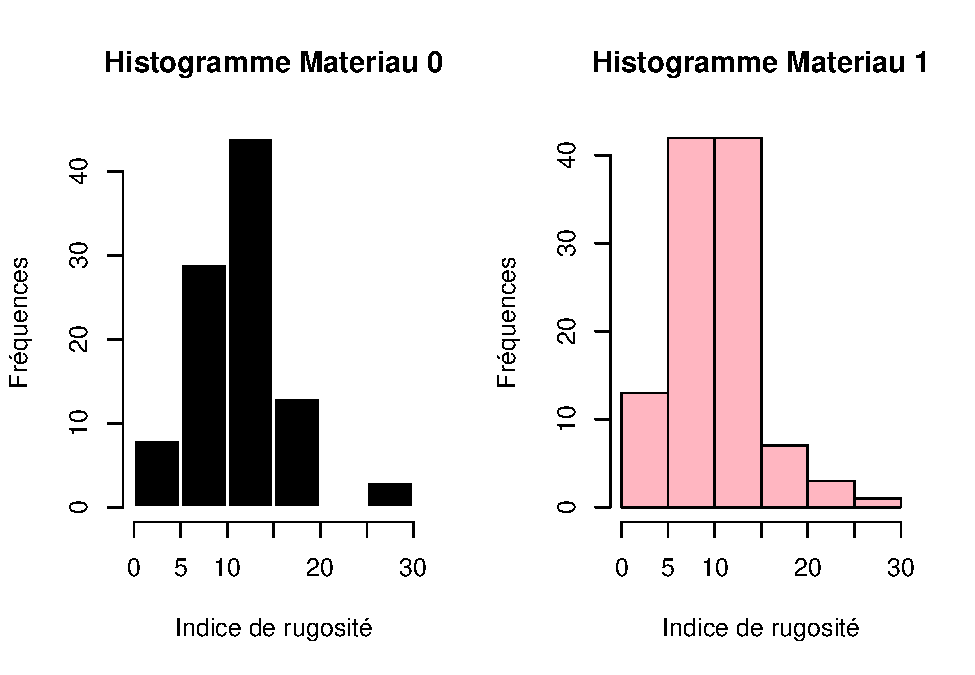
\includegraphics{devoir_files/figure-latex/unnamed-chunk-3-1.pdf}

\begin{Shaded}
\begin{Highlighting}[]
\CommentTok{\#Diagramme de Tukey}
\FunctionTok{ggplot}\NormalTok{(mondata, }\FunctionTok{aes}\NormalTok{(}\AttributeTok{y =} \FunctionTok{factor}\NormalTok{(M), }\AttributeTok{x =}\NormalTok{ IR, }\AttributeTok{fill =} \FunctionTok{factor}\NormalTok{(M))) }\SpecialCharTok{+} \FunctionTok{geom\_boxplot}\NormalTok{(}\AttributeTok{fill =} \FunctionTok{c}\NormalTok{(}\StringTok{"black"}\NormalTok{, }\StringTok{"lightpink"}\NormalTok{))}\SpecialCharTok{+} \FunctionTok{labs}\NormalTok{(}\AttributeTok{fill =} \StringTok{"Materiau"}\NormalTok{,}\AttributeTok{title =} \StringTok{"Diagramme de Tukey de l\textquotesingle{}IR par type de Materiau"}\NormalTok{, }\AttributeTok{y =} \StringTok{"type de Materiau"}\NormalTok{, }\AttributeTok{x =} \StringTok{"indice de Rugosite"}\NormalTok{)}
\end{Highlighting}
\end{Shaded}

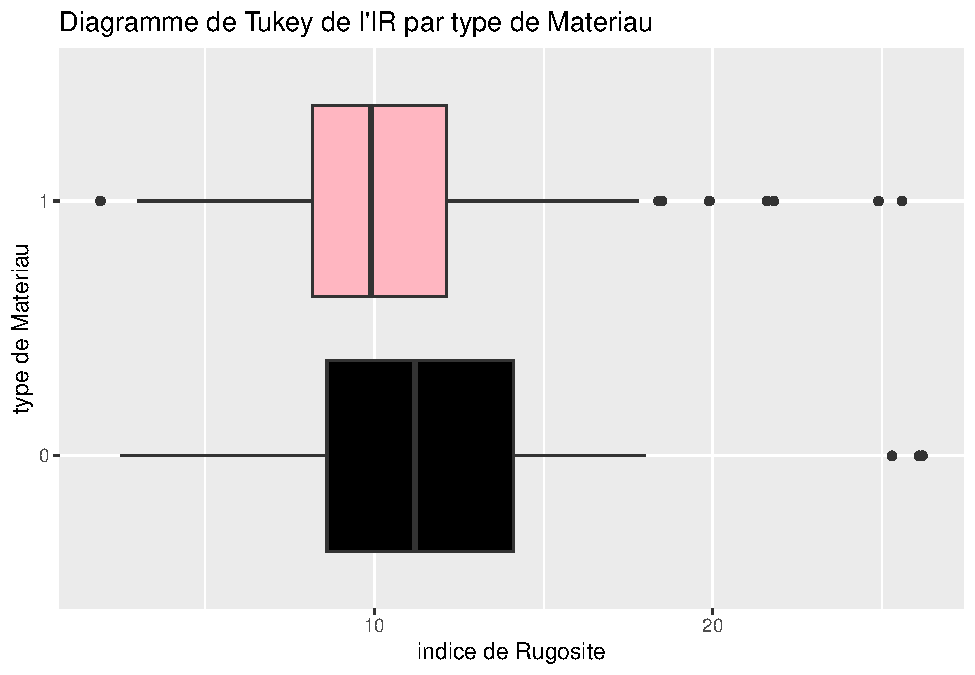
\includegraphics{devoir_files/figure-latex/unnamed-chunk-3-2.pdf}

\begin{Shaded}
\begin{Highlighting}[]
\CommentTok{\#tableau des statistiques descriptives par groupe}
\NormalTok{summary\_table }\OtherTok{\textless{}{-}}\NormalTok{ mondata }\SpecialCharTok{\%\textgreater{}\%}
  \FunctionTok{group\_by}\NormalTok{(M) }\SpecialCharTok{\%\textgreater{}\%}
  \FunctionTok{summarise}\NormalTok{(}
    \AttributeTok{moyenne =} \FunctionTok{mean}\NormalTok{(IR),}
    \AttributeTok{ecart\_type\_2 =} \FunctionTok{sd}\NormalTok{(IR),}
    \AttributeTok{q1 =} \FunctionTok{quantile}\NormalTok{(IR, }\FloatTok{0.25}\NormalTok{),}
    \AttributeTok{q2 =} \FunctionTok{quantile}\NormalTok{(IR, }\FloatTok{0.5}\NormalTok{),}
    \AttributeTok{q3 =} \FunctionTok{quantile}\NormalTok{(IR, }\FloatTok{0.75}\NormalTok{),}
    \AttributeTok{Interval\_Confiance\_Min =} \FunctionTok{t.test}\NormalTok{(IR)}\SpecialCharTok{$}\NormalTok{conf.int[}\DecValTok{1}\NormalTok{],}
    \AttributeTok{Interval\_Confiance\_Max =} \FunctionTok{t.test}\NormalTok{(IR)}\SpecialCharTok{$}\NormalTok{conf.int[}\DecValTok{2}\NormalTok{]}
\NormalTok{  )}


\NormalTok{knitr}\SpecialCharTok{::}\FunctionTok{kable}\NormalTok{(summary\_table, }\AttributeTok{caption =} \StringTok{"Tableau des statistiques descriptives sur l\textquotesingle{}indice de rugosité pour le materiau 1 et 0"}\NormalTok{)}
\end{Highlighting}
\end{Shaded}

\begin{longtable}[]{@{}
  >{\raggedleft\arraybackslash}p{(\columnwidth - 14\tabcolsep) * \real{0.0337}}
  >{\raggedleft\arraybackslash}p{(\columnwidth - 14\tabcolsep) * \real{0.1011}}
  >{\raggedleft\arraybackslash}p{(\columnwidth - 14\tabcolsep) * \real{0.1461}}
  >{\raggedleft\arraybackslash}p{(\columnwidth - 14\tabcolsep) * \real{0.0674}}
  >{\raggedleft\arraybackslash}p{(\columnwidth - 14\tabcolsep) * \real{0.0562}}
  >{\raggedleft\arraybackslash}p{(\columnwidth - 14\tabcolsep) * \real{0.0787}}
  >{\raggedleft\arraybackslash}p{(\columnwidth - 14\tabcolsep) * \real{0.2584}}
  >{\raggedleft\arraybackslash}p{(\columnwidth - 14\tabcolsep) * \real{0.2584}}@{}}
\caption{Tableau des statistiques descriptives sur l'indice de rugosité
pour le materiau 1 et 0}\tabularnewline
\toprule\noalign{}
\begin{minipage}[b]{\linewidth}\raggedleft
M
\end{minipage} & \begin{minipage}[b]{\linewidth}\raggedleft
moyenne
\end{minipage} & \begin{minipage}[b]{\linewidth}\raggedleft
ecart\_type\_2
\end{minipage} & \begin{minipage}[b]{\linewidth}\raggedleft
q1
\end{minipage} & \begin{minipage}[b]{\linewidth}\raggedleft
q2
\end{minipage} & \begin{minipage}[b]{\linewidth}\raggedleft
q3
\end{minipage} & \begin{minipage}[b]{\linewidth}\raggedleft
Interval\_Confiance\_Min
\end{minipage} & \begin{minipage}[b]{\linewidth}\raggedleft
Interval\_Confiance\_Max
\end{minipage} \\
\midrule\noalign{}
\endfirsthead
\toprule\noalign{}
\begin{minipage}[b]{\linewidth}\raggedleft
M
\end{minipage} & \begin{minipage}[b]{\linewidth}\raggedleft
moyenne
\end{minipage} & \begin{minipage}[b]{\linewidth}\raggedleft
ecart\_type\_2
\end{minipage} & \begin{minipage}[b]{\linewidth}\raggedleft
q1
\end{minipage} & \begin{minipage}[b]{\linewidth}\raggedleft
q2
\end{minipage} & \begin{minipage}[b]{\linewidth}\raggedleft
q3
\end{minipage} & \begin{minipage}[b]{\linewidth}\raggedleft
Interval\_Confiance\_Min
\end{minipage} & \begin{minipage}[b]{\linewidth}\raggedleft
Interval\_Confiance\_Max
\end{minipage} \\
\midrule\noalign{}
\endhead
\bottomrule\noalign{}
\endlastfoot
0 & 11.49381 & 4.598071 & 8.600 & 11.2 & 14.100 & 10.567098 &
12.42053 \\
1 & 10.28796 & 4.387849 & 8.175 & 9.9 & 12.125 & 9.450959 & 11.12497 \\
\end{longtable}

\#\#\#Explication: Tout d'abord, les histogrammes illustrent que la
plupart des valeurs se situent entre 5 et 15, avec des valeurs sont plus
etendues vers la droite. Cette observation est cohérente avec les
calculs des statistiques descriptives. En effet, en examinant les
moyennes, le Matériau 0 affiche une moyenne plus élevée (11.49) par
rapport au Matériau 1 (10.29), confirmant la tendance constaté. De plus,
les quartiles et les intervalles de confiance décrivent la répartition
des données, montrant que le Matériau 0 a une distribution plus étendue
que le Matériau 1. Cette conclusion est également étayée par
l'écart-type, qui est légèrement plus élevé pour le Matériau 0 (4.60)
que pour le Matériau 1 (4.39). Les observations visuelles des diagrammes
de Tukey renforcent ces résultats, suggérant que le centre du Matériau 0
est inférieur à celui du Matériau 1. De plus, bien que des données
aberrantes soient présentes dans les deux matériaux, elles semblent être
plus dispersées dans le Matériau 1. En résumé, on peut constater des
différences substantielles entre les deux matériaux que ce soit de
tendance centrale, de dispersion ou de la présence de données
aberrantes.

Avant de procéder aux tests d`hypothèses, nous allons effectuer le test
de shapiro pour verifier si l'échantillon d'IR pour les deux types de
matières suivent une loi normale:

\begin{Shaded}
\begin{Highlighting}[]
\FunctionTok{shapiro.test}\NormalTok{(matiere\_A}\SpecialCharTok{$}\NormalTok{IR)}
\end{Highlighting}
\end{Shaded}

\begin{verbatim}
## 
##  Shapiro-Wilk normality test
## 
## data:  matiere_A$IR
## W = 0.95848, p-value = 0.003767
\end{verbatim}

\begin{Shaded}
\begin{Highlighting}[]
\FunctionTok{shapiro.test}\NormalTok{(matiere\_B}\SpecialCharTok{$}\NormalTok{IR)}
\end{Highlighting}
\end{Shaded}

\begin{verbatim}
## 
##  Shapiro-Wilk normality test
## 
## data:  matiere_B$IR
## W = 0.93804, p-value = 7.851e-05
\end{verbatim}

Comme la valeur p est inférieure à 0.05 dans les deux cas (0.003767
\textless{} 0.05 et 7.851e-05 \textless\textless\textless{} 0.05), on
rejette l'hypothèse nulle selon laquelle les échantillons suivent une
distribution normale. Il est aussi possible de constater que la taille
de chaque echantillon est relativement grand:

\begin{Shaded}
\begin{Highlighting}[]
\DocumentationTok{\#\#\#\#\# Taille des echantillons}
\NormalTok{n1}\OtherTok{=}\FunctionTok{length}\NormalTok{(matiere\_A}\SpecialCharTok{$}\NormalTok{IR)}
\NormalTok{n2}\OtherTok{=}\FunctionTok{length}\NormalTok{(matiere\_B}\SpecialCharTok{$}\NormalTok{IR)}
\FunctionTok{cat}\NormalTok{(}\StringTok{"}\SpecialCharTok{\textbackslash{}n}\StringTok{Taille echantillon Materiau 0="}\NormalTok{,n1,    }\StringTok{"}\SpecialCharTok{\textbackslash{}n}\StringTok{Taille echantillon Materiau 1="}\NormalTok{,n2)}
\end{Highlighting}
\end{Shaded}

\begin{verbatim}
## 
## Taille echantillon Materiau 0= 97 
## Taille echantillon Materiau 1= 108
\end{verbatim}

\#\#\#\#Placer les formules et tout ici: \ldots{} \#\#\#Tests
d'hypothese moyenne égale:

\begin{Shaded}
\begin{Highlighting}[]
\DocumentationTok{\#\#\#\#\# test d\textquotesingle{}hypothese:}

\CommentTok{\#t.test(matiere\_A$IR,matiere\_B$IR, var.equal=FALSE)}
\CommentTok{\#test\_var \textless{}{-} var.test(matiere\_A$IR, matiere\_B$IR)}
\CommentTok{\#test\_var}
\NormalTok{Z0}\OtherTok{=}\NormalTok{(}\FunctionTok{mean}\NormalTok{(matiere\_A}\SpecialCharTok{$}\NormalTok{IR)}\SpecialCharTok{{-}}\FunctionTok{mean}\NormalTok{(matiere\_B}\SpecialCharTok{$}\NormalTok{IR))}\SpecialCharTok{/}\FunctionTok{sqrt}\NormalTok{((}\FunctionTok{var}\NormalTok{(matiere\_A}\SpecialCharTok{$}\NormalTok{IR)}\SpecialCharTok{/}\NormalTok{n1)}\SpecialCharTok{+}\NormalTok{(}\FunctionTok{var}\NormalTok{(matiere\_B}\SpecialCharTok{$}\NormalTok{IR)}\SpecialCharTok{/}\NormalTok{n2))}
\FunctionTok{cat}\NormalTok{(}\StringTok{"Z0="}\NormalTok{,Z0,}\StringTok{"}\SpecialCharTok{\textbackslash{}n}\StringTok{Zalpha/2="}\NormalTok{,}\FunctionTok{qnorm}\NormalTok{(}\FloatTok{0.05}\SpecialCharTok{/}\DecValTok{2}\NormalTok{, }\AttributeTok{lower.tail =}\NormalTok{ F))}
\end{Highlighting}
\end{Shaded}

\begin{verbatim}
## Z0= 1.915663 
## Zalpha/2= 1.959964
\end{verbatim}

Puisque Z0 \textless{} 1.959964, nous ne pouvons pas rejeter H0 à un
niveau de confiance de 95\%. Il n'y a donc pas suffisamment de preuves
statistiques pour affirmer que les moyennes des deux groupes sont
différentes. On ne peut donc pas conclure à une différence significative
entre les moyennes de matière A et matière B

\end{document}
